\section{IMPLEMENTATION}
\label{section:implementation}

\subsection{Technology Stack}
\label{sect:sub-title}
The major technology stack components used in our project are as following: Hypertext Markup Language (HTML), Cascading Style Sheets (CSS), JavaScript and
Django (High-level Python web framework).
\\
\\
For more details, the data displayed on the interface is realized by HTML and
 the style of the page is written in CSS. The back-end database construction and application interfaces are implemented by Django.
\\
\subsection{Database Construction}
\label{sect:sub-title}
\paragraph{Load Dataset}
After running the back end database on the local server, we can load the data 
by accessing the url 127.0.0.1:8000/load/. When visiting the page, the self defined function $load(request)$ will be called and load the data to the local Mysql database.  
\paragraph{Entities Construction}
Model is Django's schema for representing data. It uses Python classes as the basis for setting data items and data formats in $Models.py$, basically a database table for each class. \par
With such a class, we can define a table of a database and operate on the results of the database at an abstract level through some Settings of the table and fields. The following classes are implemented: \par
• class Customer(models.Model) \par
• class Product(models.Model) \par
• class Order(models.Model)\par
• class Address(models.Model) \par
• class customer_postal(models.Model) \par
\begin{figure}[H]
    \centering
    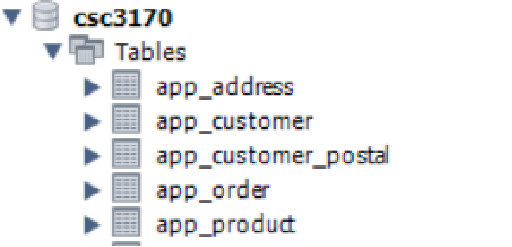
\includegraphics[width=\columnwidth/2]{images/tables.png}
    \caption[Short text]{Auto generated Mysql tables.}
    \label{fig:ER}
\end{figure}
\paragraph{Administrator Page}
Our project provides an administrator page for supermarket managers.  So that they can view, modify, delete and other operations on commodity information, customer information and order information. \par
With command line \par
$python \ manage.py \ createsuperuser$,\par
the user can create an administrator account and log in at at url 127.0.0.1:8000/admin/.  
\begin{figure}[H]
    \centering
    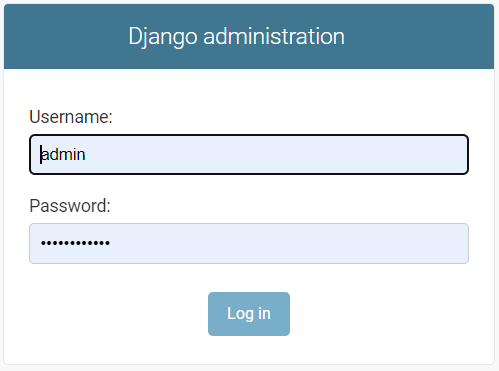
\includegraphics[width=\columnwidth/2]{images/login.png}
    \caption[Short text]{Admin login page.}
    \label{fig:ER}
\end{figure}
\begin{figure}[H]
    \centering
    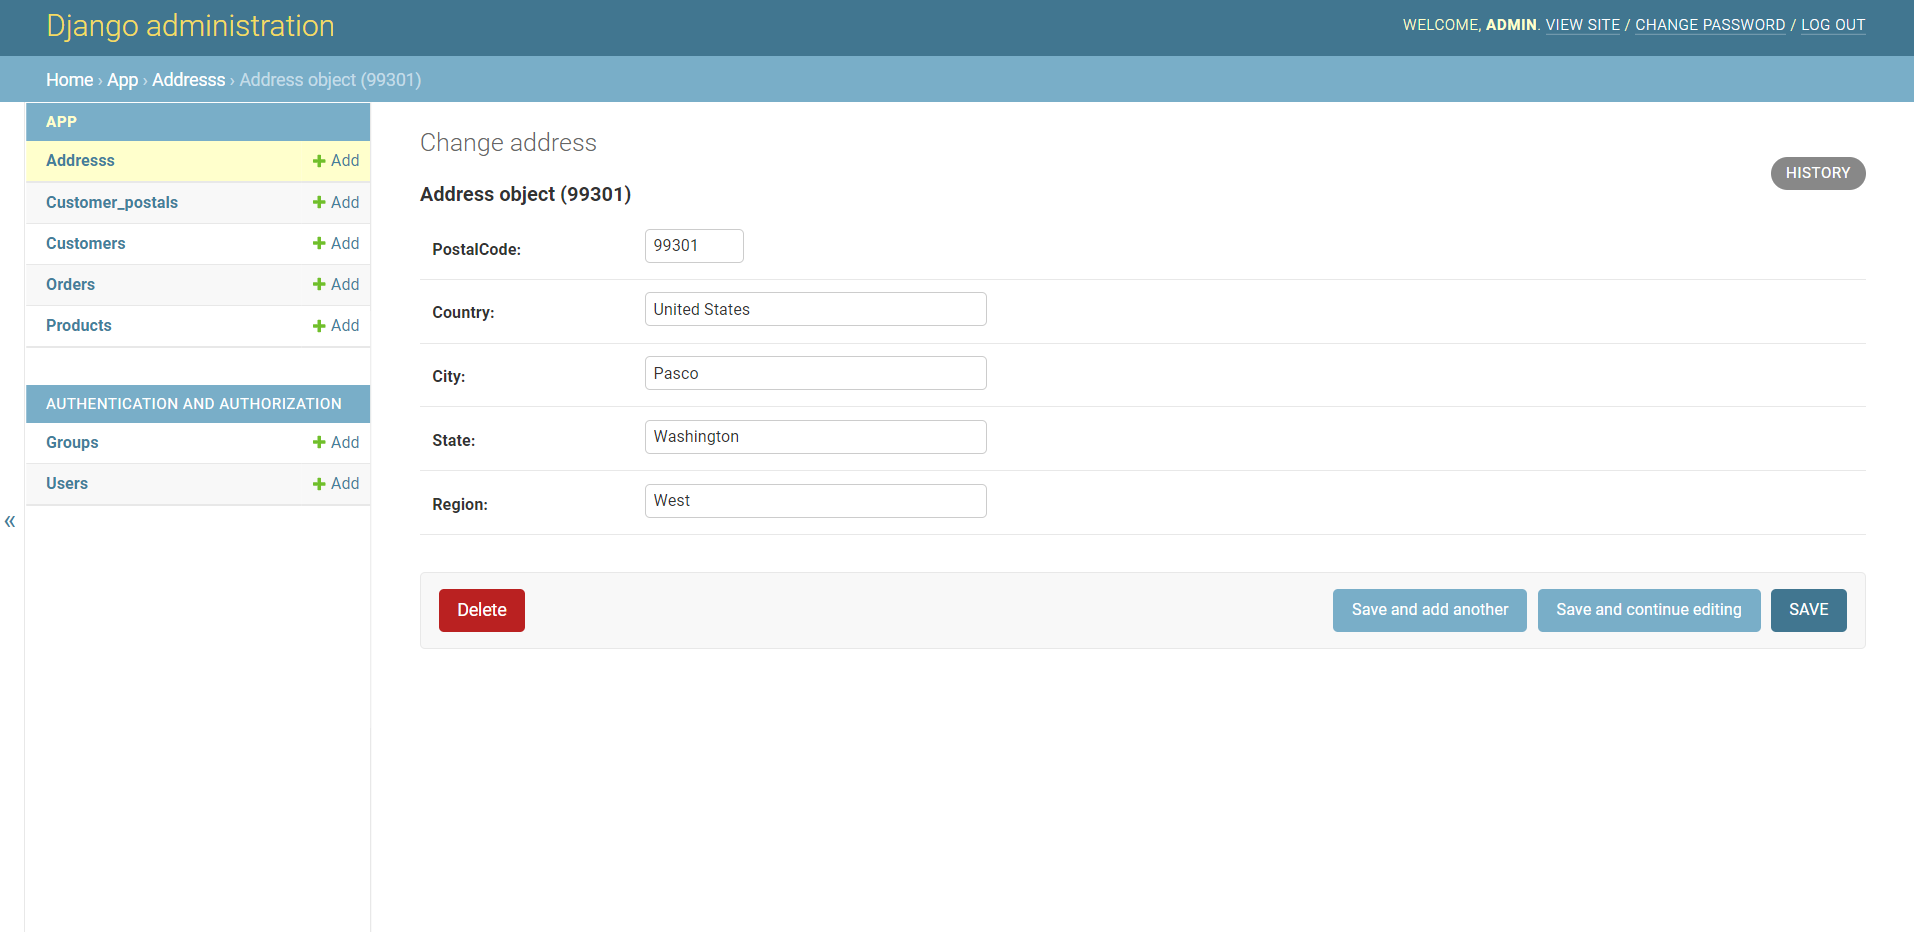
\includegraphics[width=\columnwidth]{images/admin.png}
    \caption[Short text]{Administration Page.}
    \label{fig:ER}
\end{figure}
The manager of the supermarket can change the entity to edit by clicking on the list of tables in the upper left corner of the page.  And easily manipulate the page HTML input controls to make changes to the data.  You can also add or remove data by clicking the Add or delete button.  
\paragraph{Data analysis URLs}
We set up multiple interfaces for data analysis with Django, and we can access them through the specified URL.  
\par
• $admin/$: Login to the administration page\par
• $load/$: Load data\par
• $productCount/$: Return the count of each product sold.\par
• $productProfit/$: Return the profit of each product.\par
• $categoryCount/$: Return the quantity of products from each category sold.\par
• $categoryProfit/$: Return the profit of each category.\par
• $categorySales/$: Return the sales of each category.\par
• $citySales/$: Return the sales of each city.\par
• $ShipModeCount/$: Return the count of each ship mode.\par
• $customerCount/$: Return the quantity of the products purchased by each customer.\par
• $regionCount/$: Return the quantity of the products purchased in each region.\par


\begin{figure}[H]
    \centering
    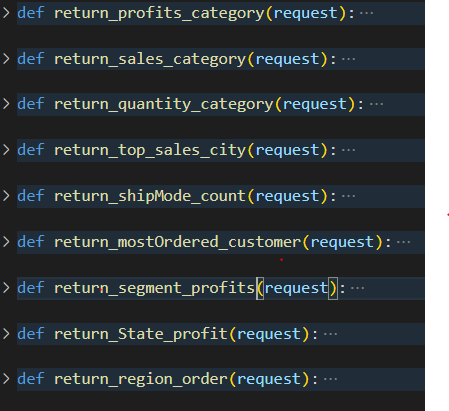
\includegraphics[width=\columnwidth]{images/functions.png}
    \caption[Short text]{Related query functions related to optional custom interfaces.}
    \label{fig:ER}
\end{figure}